\chapter{ノーデザイン: 要素,優先度,グルーピングの情報からのUI自動生成手法の提案}
\label{chap:auto-gen}

本章では,後述のiOSネイティブアプリケーションのインタフェース自動生成システムの開発に先立ち,既存のインタフェースの分析から導きさした要素,優先度,グルーピングによりインタフェースの構築が行える法則について検討した.自動生成を行うアルゴリズムの提案行う.
\section{既存インタフェースの分析}
既存のiOSネイティブアプリケーションのUIのレイアウトの分析をおこなった.数多くのUIを分析した一部としてInstagram(図\ref{fig:instagram_analyze}). Facebook(図\ref{fig:facebook_analyze}),,日経電子版(図\ref{fig:nikkei_analyze})を例に解説する.
分析の結果,画面内でのUIは画面遷移を司り,画面内の体験には直接影響を与えないUI(図\ref{fig:instagram_analyze}, 図\ref{fig:facebook_analyze}, 図\ref{fig:nikkei_analyze}左側スクリーンショット赤枠部分),画面のコンテンツを表示するUIに分類した.


\subsection{画面遷移を司るUI}
画面遷移を司るUIでは画面やアプリのタイトル,アプリ内での別機能への動線が配置されている.
AppleがiOSアプリのデザインについて定めているガイドラインであるHuman Interface Guidelines\cite{hignavigation}では,主要な画面遷移の構造としてHierarchical Navigation(図\ref{fig:hig_hierarchical}),Flat Navigation(図\ref{fig:hig_flat}),Content-Driven or Experience-Driven Navigation(図\ref{fig:hig_experiencedriven}),Content-Driven or Experience-Driven Navigation(図\ref{fig:hig_experiencedriven})が挙げられており,本分析のサンプルとなったアプリケーションではFlat Navigationの中にHierarchical Navigationがあるような構造になっている.

実際のSwiftUIにおける画面遷移を司るUIであるNavigationView\cite{appledevelopernavigationview}, TabView\cite{appledevelopertabview} でも画面遷移を司るUI,画面のタイトルとコンテンツは別で実装され,画面遷移を司るUIの上にコンテンツが乗る形式で実装されているため本研究ではそれに則り,自動生成手法の提案ではこのような画面遷移を司るUIは切り離し,画面のコンテンツのUIに注目した.


\begin{figure}[htbp]
  \begin{minipage}{\hsize}
    \begin{center}
       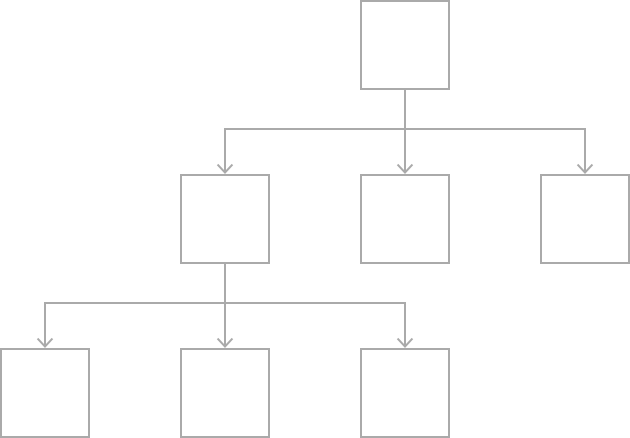
\includegraphics[width=100mm]{img/hig_hierarchical.png}
    \end{center}
    \caption{Hierarchical Navigation\cite{hignavigation}}
    \label{fig:hig_hierarchical}
  \end{minipage}
\end{figure}

\begin{figure}[htbp]
  \begin{minipage}{\hsize}
    \begin{center}
       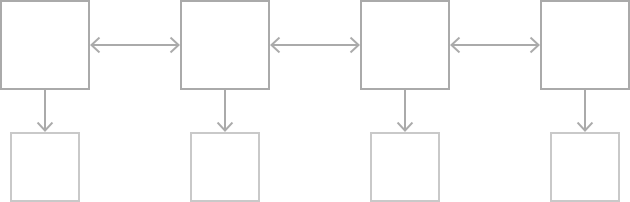
\includegraphics[width=100mm]{img/hig_flat.png}
    \end{center}
    \caption{Flat Navigation\cite{hignavigation}}
    \label{fig:hig_flat}
  \end{minipage}
\end{figure}

\begin{figure}[htbp]
  \begin{minipage}{\hsize}
    \begin{center}
       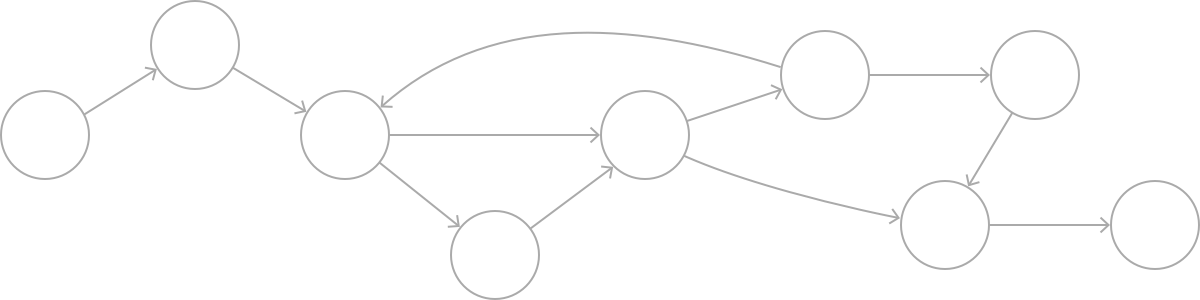
\includegraphics[width=100mm]{img/hig_ExperienceDriven.png}
    \end{center}
    \caption{Content-Driven or Experience-Driven Navigation\cite{hignavigation}}
    \label{fig:hig_experiencedriven}
  \end{minipage}
\end{figure}



\subsection{画面の内容を表示するUI}
前述では画面内のUIについて画面の内容を表示するUIを画面遷移を司るUIが内包していると述べた.本セクションでは画面の内容を表示するUIのレイアウトは主に画面内に表示する要素(UIパーツ),その要素同士の優先度,そして要素同士のグルーピングの3つのルールに則って構成されており,そのルールさえ示せば画面を構成できるのではないかという仮説を立てた.要素の種類が少ない限定的な機能を持つアプリケーションを開発する環境では,グルーピングと優先度からUIを自動生成する研究\cite{m-base} がされている.

次にレイアウトを構成する3つのルールについて述べる.
\subsubsection{要素}
画面内にどの要素がいくつ存在するのかを定める必要がある.
UI分析(図\ref{fig:instagram_analyze}, 図\ref{fig:facebook_analyze}, 図\ref{fig:nikkei_analyze})右図の灰色の長方形で要素の種類と数を表した.
\subsubsection{優先度}
画面内の要素の種類と個数がわかったら次に画面内でその要素の重要度を明確にする必要がある.
例えば,同じSNSサービスであっても写真をメインとするInstagramと文字をメインとするTwitterでは文字と画像の優先度の比重が変化する.


\subsubsection{グルーピング}
要素,優先度に加えて各要素同士でグループがある場合,グループを明確にした.
UI分析(図\ref{fig:instagram_analyze}, 図\ref{fig:facebook_analyze}, 図\ref{fig:nikkei_analyze})では緑枠,青枠がグルーピングを表した.
またグルーピングの入れ子構造では要素の表示の方向を縦方向,横方向と順に切り替えることで多くのUIが実装されていた.UI分析(図\ref{fig:instagram_analyze}, 図\ref{fig:facebook_analyze}, 図\ref{fig:nikkei_analyze})では横方向配置のグループを青枠,縦方向配置のグループを緑枠で示した.多くのUIでグループの入れ子の場合,縦横が交互に入れ替わっていることがわかる.

例外としてFacebook(図\ref{fig:facebook_analyze})上部のユーザが投稿を行う要素ではライブ,写真,Roomのボタンのグループが横に並んでいるが,写真を投稿するボタンとライブやRoomを始めるボタンが隣にあるのは機能がかけ離れているため,ユーザの誤解を招く.しかし使いやすさよりもFacebookがLive機能やRoom機能へのリーチを優先したためにこのような配置になっていると推測した.

\begin{figure}[htbp]
  \begin{minipage}{\hsize}
    \begin{center}
       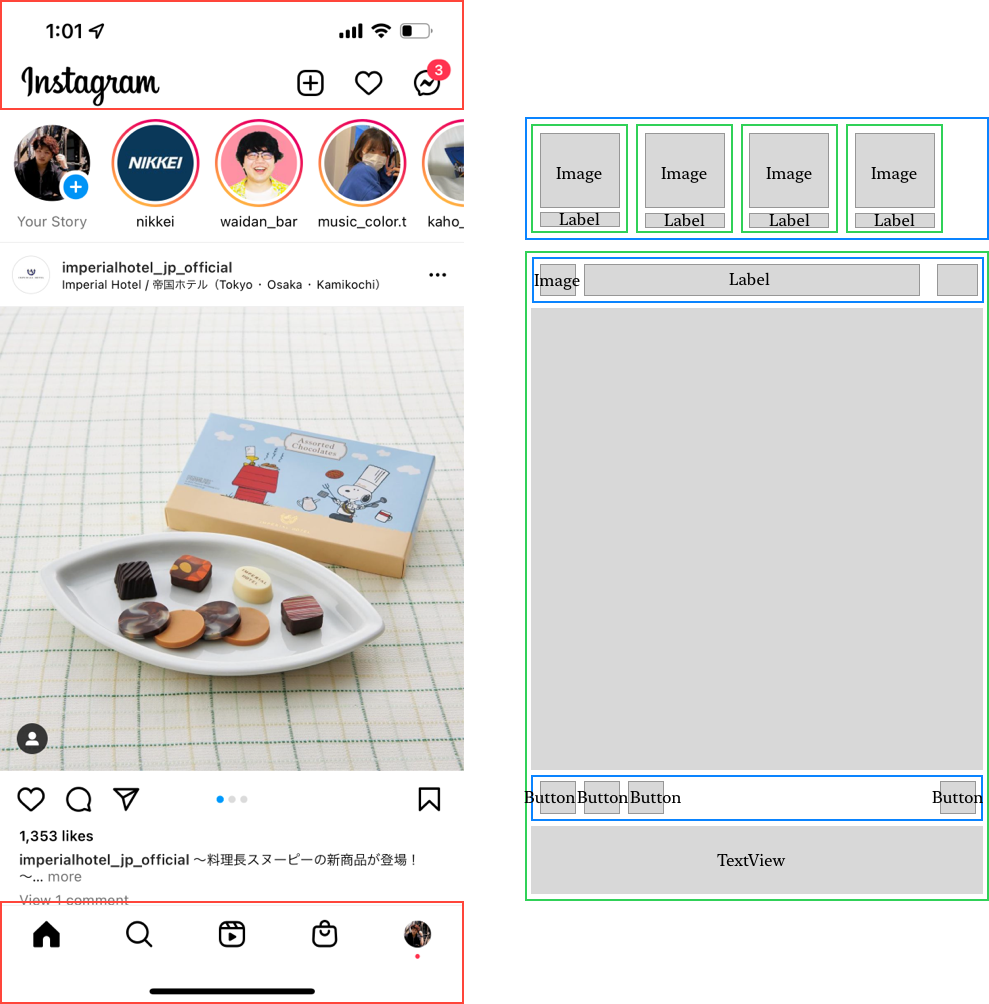
\includegraphics[width=100mm]{img/instagram_analyze.png}
    \end{center}
    \caption{InstagramiOSアプリのUIの分析}
    \label{fig:instagram_analyze}
  \end{minipage}
\end{figure}

\begin{figure}[htbp]
  \begin{minipage}{\hsize}
    \begin{center}
       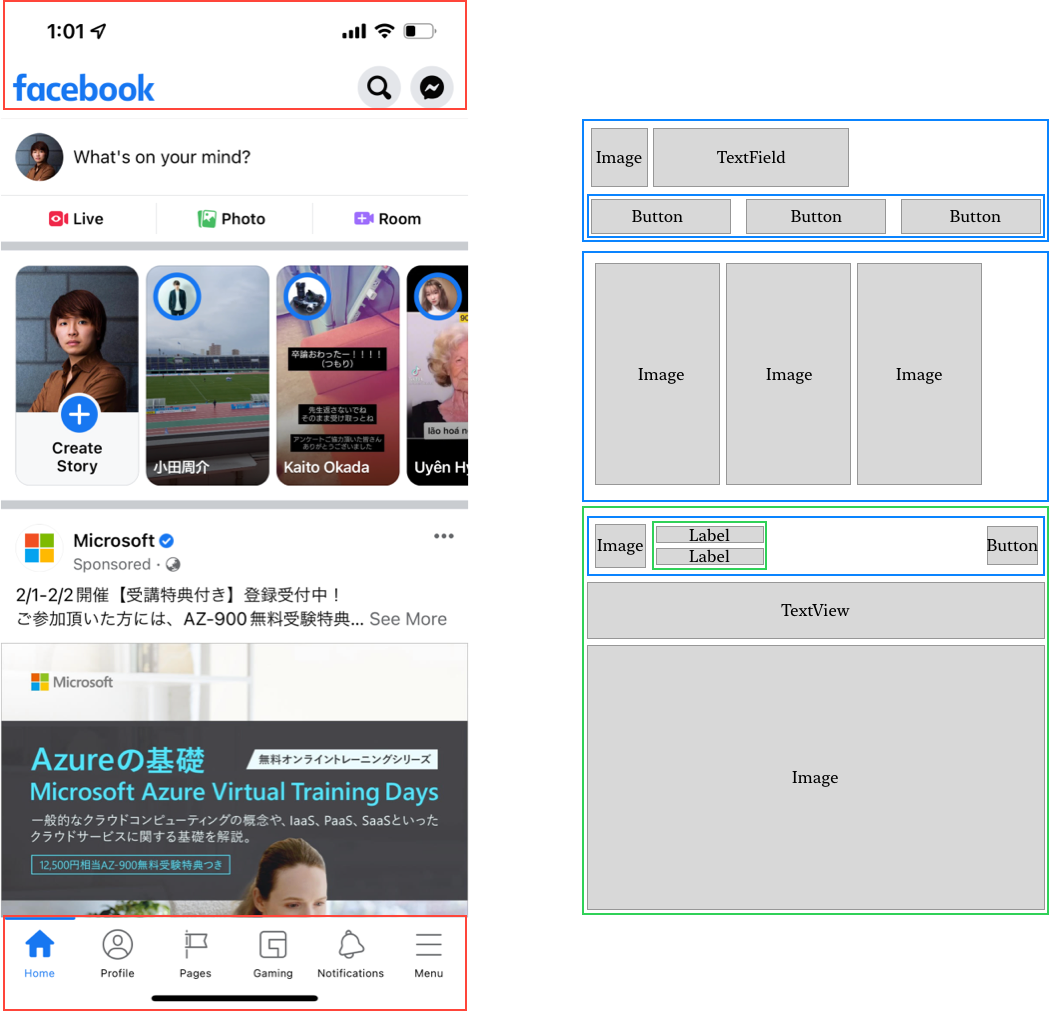
\includegraphics[width=100mm]{img/facebook_analyze.png}
    \end{center}
    \caption{facebookiOSアプリのUIの分析}
    \label{fig:facebook_analyze}
  \end{minipage}
\end{figure}

\begin{figure}[htbp]
  \begin{minipage}{\hsize}
    \begin{center}
       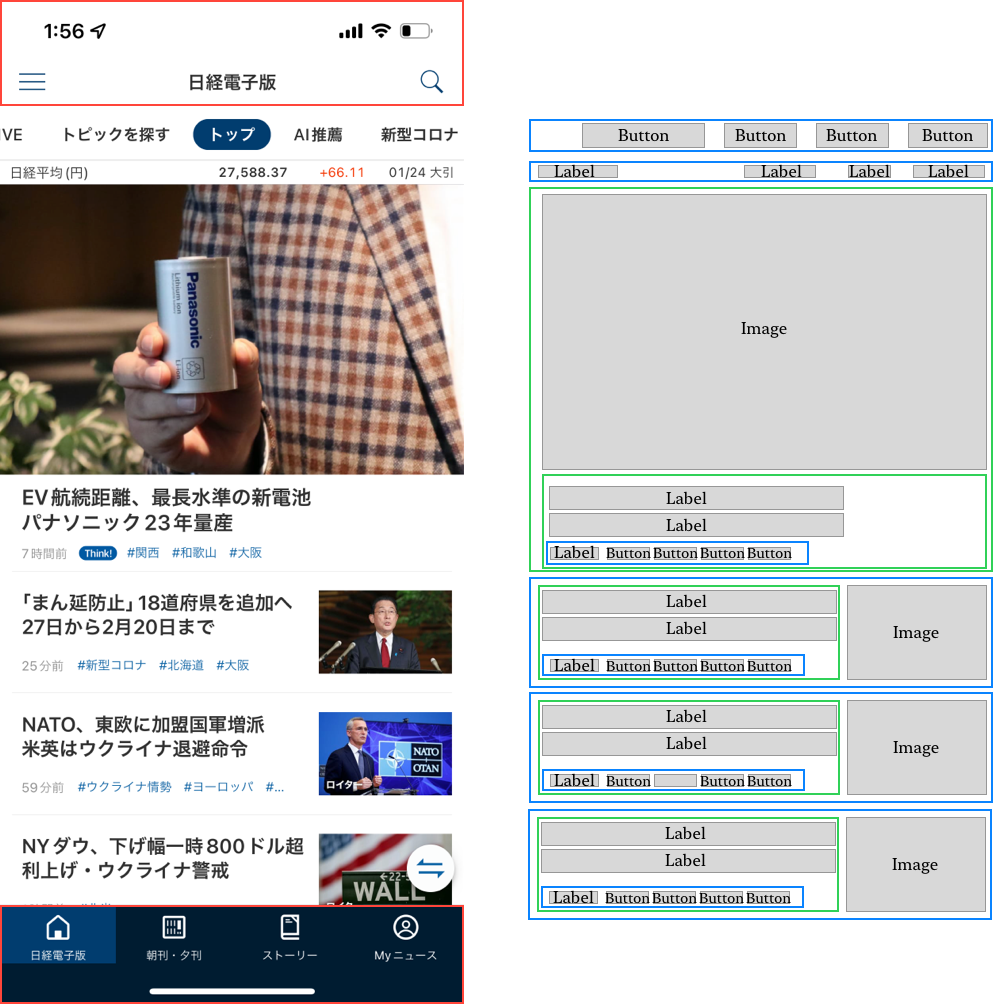
\includegraphics[width=100mm]{img/nikkei_analyze.png}
    \end{center}
    \caption{日経電子版iOSアプリのUIの分析}
    \label{fig:nikkei_analyze}
  \end{minipage}
\end{figure}

\section{アルゴリズムの構築}
次にこの要素,要素同士の優先度,要素のグルーピングから1画面のUIを構成するアルゴリズムを検討した.
要素を優先度の高い順に画面内に縦に並べることを基本とし,グループは一つの要素として配置する.また,グループの優先度はグループ内の要素の優先度の合計とした.
しかしながら,要素の中にはユーザが操作するもの,見るだけのものがあり,操作するものは指の届きやすい画面下部に配置するのが適切である.各要素の種類に応じて別途配置係数を定め,配置係数と優先度を組み合わせて画面内に配置する場所を決定する必要がある.
Groupが入れ子になる場合はHstack, Vstackを交互にすることによってUIを構成する.
画面内の要素の優先度の基準を10とし,それを超える場合はスクロールするようにする.
優先度が上がる度に文字は大きく,太く,ボタンもただの青文字ではなく,borderがついたり,塗り領域が増えたりと視覚的にも目立たせることで優先度をより効果的に扱う.

